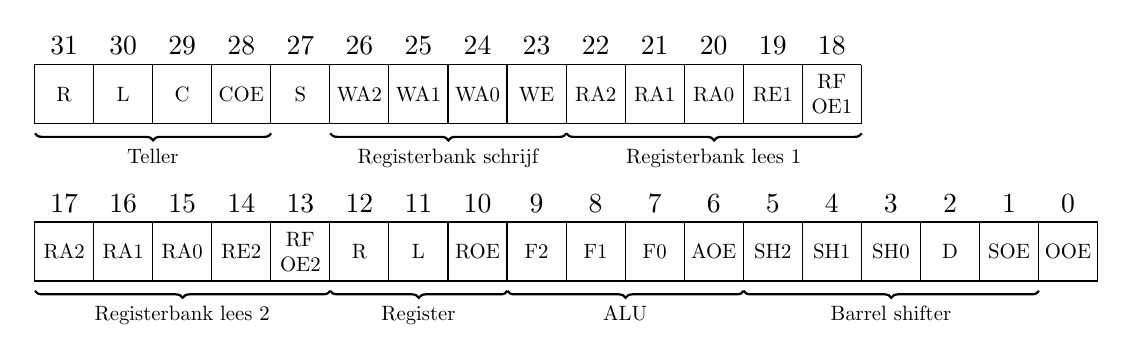
\begin{tikzpicture}
\foreach \j/\xa/\xb/\b/\g in {0/31/18/{31/R,30/L,29/C,28/COE,27/S,26/WA2,25/WA1,24/WA0,23/WE,22/RA2,21/RA1,20/RA0,19/RE1,18/{RF\\OE1}}/{31/28/Teller,26/23/Registerbank schrijf,22/18/Registerbank lees 1},-2/17/0/{17/RA2,16/RA1,15/RA0,14/RE2,13/{RF\\OE2},12/R,11/L,10/ROE,9/F2,8/F1,7/F0,6/AOE,5/SH2,4/SH1,3/SH0,2/D,1/SOE,0/OOE}/{17/13/Registerbank lees 2,12/10/Register,9/6/ALU,5/1/Barrel shifter}} {
  \begin{scope}[yshift=\j cm]
	\begin{scope}[xshift=0.75*\xa cm]
	\foreach \i/\t in \b {
	  \begin{scope}[xshift=-0.75*\i cm]
		\node[scale=0.75] (I-\i) at (0,0) {\begin{minipage}{1.0 cm}\begin{center}\t\end{center}\end{minipage}};
		\draw (0.375,0.375) -- ++(0,-0.75);
		\draw (0,0.375) node[anchor=south] {$\i$};
	  \end{scope}
	}
	\foreach \ya/\yb/\t in \g {
	  \draw[thick,decorate,decoration={brace,mirror}] (-0.37-0.75*\ya,-0.5) -- (0.38-0.75*\yb,-0.5);
	  \draw (-0.375*\yb-0.375*\ya,-0.6) node[anchor=north,scale=0.75] {\t};
	}
	\end{scope}
	\draw (0.75*\xa-0.75*\xb+0.375,0.375) -- (-0.375,0.375) -- (-0.375,-0.375) -- (0.75*\xa-0.75*\xb+0.375,-0.375);
  \end{scope}
}
\end{tikzpicture}